\documentclass[13pt, letterpaper]{article}
\usepackage{graphicx}
\usepackage{multirow}
\graphicspath{{assets}}

\title{\textbf{A big page}}
\author{Milinda Barua}
\date{20th October 2024}
\begin{document}
\maketitle
\begin{figure}[h]
    \centering
    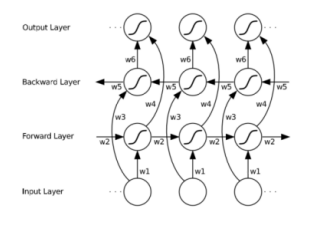
\includegraphics[width=0.5\linewidth]{./assets/image1.png}
    \caption{An image caption}
    \label{fig:label}
\end{figure}
As you can see in figure \ref{fig:label}, the function grows near the origin. This example is on page \pageref{fig:label}.

\begin{itemize}
    \item This is the first item
    \item This is the second item
    \item This is the third item
\end{itemize}

\begin{enumerate}
    \item This is the first item
    \item This is the second item
    \item This is the third item
\end{enumerate}

In physics, the mass-energy equivalence is stated
by the equation $E=mc^2$, discovered in 1905 by Albert Einstein.

\begin{math}
    \newline
    E=mc^2
    \newline
    b^2 - 4ac = 0
\end{math} is typeset in a paragraph using inline math mode---as is $E=mc^2$, and so too is \(E=mc^2\).

\begin{equation}
    E=mc^2
    b^2 - 4ac = 0
    \delta
    \alpha
\end{equation}
\newline
$\delta$
\newline
$\alpha$
\newline

hello there
this is a \LaTeX{} document
this is a second \LaTeX{} document


\begin{table}[h!]
    \centering
    % \begin{tabular}{|c|c|c|}
    \begin{tabular}{|p{3cm}|p{3cm}|p{3cm}| }
        \hline
        Country Name or Area Name & ISO ALPHA 2 Code & ISO ALPHA 3 Code \\
        \hline
        Afghanistan               & AF               & AFG              \\
        Aland Islands             & AX               & ALA              \\
        \hline
        Albania                   & AL               & ALB              \\
        Algeria                   & DZ               & DZA              \\
        American Samoa            & AS               & ASM              \\
        Andorra                   & AD               & AND              \\
        Angola                    & AO               & AGO              \\
        \hline
    \end{tabular}
    \label{tab:my_label}
\end{table}

\begin{table}[h!]
    \centering
    \begin{tabular}{c c}
        Table:                             & row table              \\
        \hline
        \textbf{first column}              & \textbf{second column} \\
        \multirow{2}{*}{\textbf{Multirow}} & X                      \\
                                           & X                      \\
        Cricket                            & Football               \\
        \hline
    \end{tabular}
\end{table}

\subsection{List}
\begin{enumerate}
    \item first item
          \begin{itemize}
              \item apple
              \item mango
          \end{itemize}
    \item second item
          \begin{itemize}
              \item car
              \item bike
          \end{itemize}
\end{enumerate}

\end{document}